\documentclass[11pt]{article}
\usepackage[a4paper,margin=25mm]{geometry}
\usepackage[T1]{fontenc}
\usepackage{lmodern,microtype,amsmath,amssymb,mathtools,booktabs,tabularx,array,xcolor,enumitem,graphicx}
\renewcommand{\tabularxcolumn}[1]{>{\raggedright\arraybackslash}p{#1}}
\usepackage[hidelinks]{hyperref}
\usepackage[backend=biber,style=numeric,sorting=none,maxbibnames=8]{biblatex}
\addbibresource{references.bib}
\addbibresource{../../unpublished-papers.bib}
\setlength{\emergencystretch}{3em}
\sloppy
\definecolor{prospectivered}{RGB}{185,0,0}
\newenvironment{prospective}{\color{prospectivered}}{}

\title{\textbf{Compatibility of Spectral and Operator Reductions\\of a First-Principles Silicon Hamiltonian}}
\author{Eugene Joseph M. Ragasa\\Department of Physics, De La Salle University, Manila, Philippines\\\texttt{eugene.ragasa@dlsu.edu.ph}}
\date{Pre-results working manuscript}
\begin{document}
\maketitle
\begin{prospective}
\noindent\textbf{Working-color convention.} Red text identifies planned production work,
open controls, pending evidence, or conditional conclusions. Black numerical content in
the appendices is bounded historical evidence and is not production silicon evidence.
\end{prospective}
\begin{prospective}
\begin{abstract}
First-principles Hamiltonians can be reduced to compact lattice models by fitting
selected spectra or by approximating an aligned localized operator. These objectives
constrain different information and need not select the same Hamiltonian. This paper
defines a first-principles bulk-silicon test of their compatibility within a nested
hierarchy of orthogonal ten-orbital $sp^3s^\ast$ Slater--Koster models. The intended
common parent is a numerically qualified, non-spin-polarized, non-spin--orbit-coupled PBE
Kohn--Sham calculation represented in a validated Wannier basis. A spectral loss
constrains training bands and declared band-edge observables. A normalized operator loss
compares real-space hopping matrices after an explicit space-group-compatible orbital
alignment and finite-domain tail gate. The two losses define spectral and operator
admissible sets. A common feasible witness supports compatibility; certified lower and
feasible upper bounds on their minimum distance distinguish class-relative
incompatibility from an inconclusive search. This pre-results manuscript reports no
production silicon compatibility or model-selection conclusion.
\end{abstract}
\noindent\textbf{Keywords:} model selection; operator compatibility; silicon;
tight-binding reduction; Wannier Hamiltonian
\end{prospective}

\section{Introduction}
Density-functional theory (DFT) supplies a first-principles Kohn–Sham description of crystalline electronic structure~\cite{hohenberg1964,kohn1965}. Plane waves provide a systematic periodic representation but are inconvenient for interpolation, large cells, and local model construction. Maximally localized Wannier functions transform a selected Kohn–Sham subspace into a localized representation whose real-space matrix elements support interpolation~\cite{marzari2012,souza2001,pizzi2020,yates2007}. Parameterized tight-binding models impose a smaller basis, finite hopping range, and symmetry structure~\cite{slater1954,vogl1983}. This additional restriction introduces model-reduction error.

A band fit and an operator reduction answer different questions. Eigenvalues do not uniquely determine eigenvectors, orbital coordinates, onsite matrices, or hopping blocks. Models with similar selected bands can therefore differ as represented operators. Conversely, a small matrix residual under one weighting does not guarantee accurate valley curvature or other band-edge observables. Neither criterion should be used as an undeclared substitute for the other.

An operator comparison is meaningful only after the state spaces are identified. The Wannier and tight-binding matrices must share compatible dimensions, orbital content, lattice translations, units, energy reference, and coordinate ordering. Their remaining coordinate freedom must be related by an admissible alignment map. Polar decomposition and principal-angle methods support alignment diagnostics~\cite{bjorck1973,higham1986}, but a small residual alone does not prove that a map respects the silicon space group or orbital semantics.

This paper asks whether spectral and operator requirements admit a common reduced silicon Hamiltonian in a prescribed class. Instead of comparing two isolated best fits, it defines the complete sets accepted by each criterion. If those sets intersect, a common witness satisfies both reductions. If they are certified to be disjoint, their minimum separation measures a class-relative obstruction. Failure to find an intersection without such a certificate remains inconclusive.

The physical branch is restricted to pristine bulk silicon in a scalar-relativistic, non-spin-polarized, non-SOC treatment. Experimental agreement is not an independent fit target. All reduction errors are relative to the selected PBE/Wannier parent. Consequently, even a compatible result would not remove parent-model discrepancy or establish transfer to defects, optical response, strain, transport, or another physical branch.

Companion controlled-model manuscripts verify common-space transport, hopping
reconstruction, finite-range reduction, gauge attacks, and changed fitting objectives
in synthetic systems~\cite{Ragasa2026a,Ragasa2026b,Ragasa2026c}. Those results motivate
this application but cannot select or validate silicon settings. Common-space defect
construction, obstruction analysis, and SOC dopant applications remain separate
unpublished works~\cite{Ragasa2026e,Ragasa2026f,Ragasa2026g}.
Appendix~\ref{app:tutorial} separately preserves a read-only
Wannier90 silicon tutorial preview: it verifies one same-frame represented-operator
decomposition and a negative 57-of-64-block truncation test, but it is excluded from the
production admissible sets.

\begin{prospective}
\section{Methodology}
\subsection{First-principles parent and reference}
The planned production parent fixes the crystal structure, exchange–correlation functional, pseudopotential, spin treatment, and numerical settings. It uses Quantum ESPRESSO~\cite{giannozzi2009}, the Perdew--Burke--Ernzerhof
generalized gradient approximation~\cite{perdew1996}, and an optimized norm-conserving
pseudopotential from the PseudoDojo family~\cite{hamann2013,vansetten2018}. The exact executable, pseudopotential content hash, lattice, cutoffs, reciprocal mesh, convergence tolerances, retained bands, and runtime environment form the immutable parent identity.

The converged self-consistent density defines the Kohn–Sham potential. Subsequent non-self-consistent and band calculations solve

\begin{equation*}
\hat H_{\mathrm{KS}}[n_{\mathrm{SCF}}]\psi_{n\mathbf k}
=
\epsilon_{n\mathbf k}\psi_{n\mathbf k}.
\tag{1}
\end{equation*}
Density convergence, band-path visualization, valley location, local effective-mass extraction, and Wannier construction use distinct wavevector designs. Numerical convergence is judged against downstream quantities rather than total energy alone. The retained observables include fixed-point band energies, indirect Kohn–Sham gap, valley coordinate, longitudinal mass, and both unaveraged transverse masses.

\subsection{Wannier representation and real-space support}
A ten-orbital target subspace contains the valence and low conduction states needed for the silicon valley analysis. Its Wannier matrix elements are

\begin{equation*}
[\mathbf H_{\mathrm W}(\mathbf R)]_{\alpha\beta}
=
\left\langle w_{\alpha\mathbf0}\middle|
\hat H_{\mathrm{KS}}
\middle|w_{\beta\mathbf R}\right\rangle.
\tag{2}
\end{equation*}
Initial projections, separately declared frozen and outer windows, reciprocal mesh, centers, spreads, and real-space inventory are part of the representation identity. Direct-parent and interpolated Wannier eigenvalues are compared on wavevectors excluded from construction. Unresolved subspace identity, gauge, decay, or projection/window sensitivity stops the operator analysis.

The comparison domain $\mathcal S_H$ is drawn from the complete retained translation inventory $\mathcal S_{\mathrm{all}}$. The excluded squared operator-norm fraction is

\begin{equation*}
\varepsilon_{\mathrm{tail}}^2(\mathcal S_H)
=
\frac{
\displaystyle\sum_{\mathbf R\in
\mathcal S_{\mathrm{all}}\setminus\mathcal S_H}
\omega_{\mathbf R}\|\mathbf H_{\mathrm W}(\mathbf R)\|_{\mathrm F}^2
}{
\displaystyle\sum_{\mathbf R\in\mathcal S_{\mathrm{all}}}
\omega_{\mathbf R}\|\mathbf H_{\mathrm W}(\mathbf R)\|_{\mathrm F}^2
}.
\tag{3}
\end{equation*}
This is not a physical energy fraction and does not prove decay beyond the represented Wannier mesh. The domain is enlarged until the diagnostic is stable and its square is below a separately frozen threshold $\tau_{\mathrm{tail}}$.

\subsection{Orbital alignment contract}
A unitary map $\mathbf C$ transforms tight-binding coordinates into Wannier coordinates. The admissible family $\mathcal U$ is not unrestricted $U(10)$. It binds site identity, orbital semantics, centers, and authenticated representations of retained symmetry operations. Every map must satisfy

\begin{equation*}
\mathbf C\mathbf D_{\mathrm{TB}}(g)
=
\mathbf D_{\mathrm W}(g)\mathbf C,
\qquad g\in G_{\mathrm{bind}}.
\tag{4}
\end{equation*}
The symbol $\mathbf D(g)$ includes the declared action of fractional translations, sublattice permutations, cell relabeling, and wavevector phases where applicable. Equation (4) is only a constraint. Calling it a realization of $Fd\bar{3}m$ additionally requires the two space-group representations, origins, translations, and induced maps to be independently constructed and authenticated.

The frozen family may contain declared site/orbital permutations, phases in one- dimensional blocks, and block-unitary transformations inside explicit equivalent multiplicity spaces. It prohibits mixing incompatible sites, irreducible representations, or orbital-semantic classes unless that freedom is justified and predeclared. Principal angles, intertwining residuals, singular values, alignment nonuniqueness, and initialization stability are retained separately from operator approximation error.

\subsection{Losses and admissible sets}
Each candidate class $\mathfrak M_j$ fixes its canonical parameter vector $\boldsymbol\theta$, orbital semantics, neighbor shells, and symmetry constraints. The planned hierarchy begins with a nearest-neighbor orthogonal ten-orbital $sp^3s^\ast$ class and adds longer-range or selected symmetry-allowed terms in a frozen sequence.

The dimensionless spectral loss is

\begin{equation*}
\mathcal L_E(\boldsymbol\theta)
=
\sum_{n,\mathbf k}w_{n\mathbf k}
\left|
\frac{\epsilon_{n\mathbf k}^{\mathrm{TB}}(\boldsymbol\theta)
-\epsilon_{n\mathbf k}^{\mathrm W}}{s_{n\mathbf k}}
\right|^2
+
\sum_m w_m
\left|
\frac{O_m^{\mathrm{TB}}(\boldsymbol\theta)-O_m^{\mathrm W}}{s_m}
\right|^2.
\tag{5}
\end{equation*}
Training and withheld points, band identities, observable components, weights, and nonzero scales are frozen before fitting. Longitudinal and two transverse masses remain separate components.

The normalized operator loss is

\begin{equation*}
\mathcal L_H(\mathbf C,\boldsymbol\theta)
=
\frac{
\displaystyle\sum_{\mathbf R\in\mathcal S_H}\omega_{\mathbf R}
\left\|\mathbf H_{\mathrm W}(\mathbf R)
-\mathbf C\mathbf H_{\mathrm{TB}}(\mathbf R;\boldsymbol\theta)
\mathbf C^\dagger\right\|_{\mathrm F}^{2}
}{
\displaystyle\sum_{\mathbf R\in\mathcal S_H}\omega_{\mathbf R}
\left\|\mathbf H_{\mathrm W}(\mathbf R)\right\|_{\mathrm F}^{2}
}.
\tag{6}
\end{equation*}
The tight-binding matrix is zero on comparison-domain translations outside its model support. Long-range parent terms therefore remain visible rather than being silently aliased into shorter-range parameters. Residuals are also reported by onsite/hopping role, orbital block, symmetry channel, and neighbor shell.

The admissible sets are

\begin{equation*}
\mathfrak A_{E,j}
=
\{\mathbf H(\boldsymbol\theta)\in\mathfrak M_j:
\mathcal L_E(\boldsymbol\theta)\leq\tau_E\},
\tag{7}
\end{equation*}
and

\begin{equation*}
\mathfrak A_{H,j}
=
\{\mathbf H(\boldsymbol\theta)\in\mathfrak M_j:
\min_{\mathbf C\in\mathcal U}\mathcal L_H(\mathbf C,\boldsymbol\theta)
\leq\tau_H\}.
\tag{8}
\end{equation*}
Threshold-derivation rules are declared before production evidence is inspected. Their final values may reflect demonstrated numerical and extraction floors, but are frozen before compatibility fitting and are not retuned after model outcomes are known.

\subsection{Separation, validation, and model selection}
Canonical parameter scales $s_q$ and weights $v_q$ define

\begin{equation*}
d_{\mathrm{TB}}(\boldsymbol\theta_1,\boldsymbol\theta_2)
=
\left[
\sum_qv_q
\left(\frac{\theta_{1,q}-\theta_{2,q}}{s_q}\right)^2
\right]^{1/2}.
\tag{9}
\end{equation*}
The minimum separation and numerical bounds are

\begin{equation*}
\delta_j^\ast
=
\inf_{\substack{
\mathbf H(\boldsymbol\theta_E)\in\mathfrak A_{E,j}\\
\mathbf H(\boldsymbol\theta_H)\in\mathfrak A_{H,j}}}
 d_{\mathrm{TB}}(\boldsymbol\theta_E,\boldsymbol\theta_H),
\tag{10}
\end{equation*}
and

\begin{equation*}
0\leq\underline\delta_j\leq\delta_j^\ast\leq\overline\delta_j.
\tag{11}
\end{equation*}
A common feasible witness supports compatibility. A feasible pair provides an upper bound; multistart optimization alone does not certify the lower bound. A certified lower bound above the map resolution supports incompatibility only within the frozen class and domain. Otherwise the result is inconclusive.

Withheld evidence includes excluded band energies, the indirect gap, valley coordinate, longitudinal mass, both transverse masses, and declared operator blocks or translations. Mass observations require identity-tracked nondegenerate branches and stable primary/ guard stencils before entering a loss. Stencil variation is local-extraction error and is not hidden by enlarging $\tau_E$.

The decision keeps four channels separate: parent-model discrepancy, numerical/discretization error, local-extraction error, and model-reduction error. The first hierarchy member with a verified compatibility witness and passing withheld gates is selected. Missing, conflicting, or ill-conditioned required evidence produces an inconclusive disposition.

\end{prospective}
\begin{prospective}
\section{Results and discussion}
\subsection{Current production evidence boundary}
No production silicon result is reported in this working draft. The project has not yet accepted, for this paper, a production lattice and Kohn–Sham parent, a numerically qualified ten-orbital Wannier operator, authenticated silicon symmetry intertwiners, complete spectral and operator admissible sets, a compatibility witness, certified separation bounds, or withheld effective masses. Consequently, this draft contains no silicon parameter table, accepted mass values, or model-selection conclusion.

This absence is an evidence boundary rather than a numerical result. Successful software tests, controlled toy-model calculations, tutorial runs, and proposed thresholds cannot substitute for the production gates. The bounded tutorial values in Appendices C and D remain historical software/numerical evidence, not production silicon results.

\subsection{Permitted future outcomes}
When authenticated evidence becomes available, Table 1 governs its interpretation.

\textbf{Table 1. Decision logic for one frozen silicon candidate class.}

\begin{center}\small
\begin{tabularx}{\textwidth}{XXX}
\toprule
\textbf{Evidence} & \textbf{Supported interpretation} & \textbf{Unsupported interpretation} \\
\midrule
Common feasible witness and passed withheld gates & Compatible within the frozen protocol & Experimental accuracy or universal transferability \\
$\overline\delta_j$ below map resolution & Resolution-limited compatibility & Proof of exact continuous-set intersection \\
Certified $\underline\delta_j$ above map resolution & Incompatible within the frozen class and domain & Failure of tight binding in general \\
Separated samples without a lower-bound certificate & Inconclusive & Proof of disjoint admissible sets \\
Failed parent, Wannier, alignment, or extraction gate & Inconclusive & Permission to relax or omit that gate \\
\bottomrule
\end{tabularx}
\end{center}
A nearest-neighbor failure would identify a limitation of that model class under the frozen basis, range, symmetry, domain, and tolerances. It would not establish that all tight-binding descriptions fail. Conversely, a compatible model would remain relative to the selected PBE/Wannier parent and would not validate unmeasured response functions.

\subsection{Results reserved for authenticated evidence}
The eventual results section will report parent convergence, direct/Wannier withheld bands, real-space tail convergence, alignment diagnostics, admissible-set evidence, separation bounds, withheld band-edge observables, and residual attribution. Training and withheld quantities will appear separately. Failed and inconclusive hierarchy members will be retained rather than omitted.

The empty records in Appendix~\ref{app:pending} define the required fields. They are not
estimates or implied findings.

\end{prospective}
\begin{prospective}
\section{Conclusions and recommendations}
The proposed silicon test treats spectral and operator reduction as a common-model problem. It requires a qualified first-principles parent, validated localized representation, symmetry-constrained alignment, independently normalized losses, controlled real-space support, bounded set-separation evidence, and withheld observables. This structure prevents band agreement, matrix agreement, numerical convergence, and material validity from being conflated.

No production compatibility conclusion follows from the present draft. The scientific result must remain withheld until all prerequisite and validation gates have produced authenticated evidence. If completed, the method will select the smallest tested class that satisfies both criteria, report a certified class-relative obstruction, or return an inconclusive result without post-hoc threshold relaxation.

\end{prospective}
\section{Nomenclature}
\begin{center}\small
\begin{tabularx}{\textwidth}{XXX}
\toprule
\textbf{Symbol} & \textbf{Description} & \textbf{Unit} \\
\midrule
$\mathfrak A_E,\mathfrak A_H$ & Spectral and operator admissible sets & — \\
$\mathbf C$ & Orbital-coordinate alignment & — \\
$\mathbf D(g)$ & Representation of symmetry operation $g$ & — \\
$d_{\mathrm{TB}}$ & Canonical tight-binding parameter distance & — \\
DFT & Density-functional theory & — \\
$\mathbf H_{\mathrm{KS}}$ & Kohn–Sham Hamiltonian & energy \\
$\mathbf H_{\mathrm W}(\mathbf R)$ & Wannier real-space Hamiltonian & energy \\
$\mathbf H_{\mathrm{TB}}(\mathbf R)$ & Tight-binding real-space Hamiltonian & energy \\
$\mathcal L_E,\mathcal L_H$ & Spectral and operator losses & dimensionless \\
$\mathfrak M_j$ & Candidate tight-binding model class & — \\
NSCF & Non-self-consistent field & — \\
PBE & Perdew–Burke–Ernzerhof approximation & — \\
$\mathcal S_H$ & Operator-comparison translation domain & — \\
SCF & Self-consistent field & — \\
SOC & Spin–orbit coupling & — \\
$\boldsymbol\theta$ & Canonical tight-binding parameters & mixed \\
$\tau_E,\tau_H,\tau_{\mathrm{tail}}$ & Frozen thresholds & dimensionless \\
$\delta_j^\ast$ & Minimum admissible-set separation & — \\
$\underline\delta_j,\overline\delta_j$ & Lower and upper separation bounds & — \\
$\varepsilon_{\mathrm{tail}}$ & Retained-inventory operator-norm tail diagnostic & — \\
$\mathcal U$ & Admissible alignment family & — \\
\bottomrule
\end{tabularx}
\end{center}
\begin{prospective}
\section{Acknowledgments}
\textbf{Author action before submission.} Add verified funding, computing-resource, institutional, and technical acknowledgments.

\end{prospective}
\printbibliography[title={References}]

\clearpage
\appendix
\begin{prospective}
\section{Planned protected calculation sequence}\label{app:plan}
This appendix records proposed work. It does not authorize calculator execution.

Before execution, the campaign must bind an accepted production-lattice artifact, authenticated full-precision inputs, exact executable and pseudopotential identities, the physical branch, numerical settings, warning and stop policies, stage manifests, and explicit execution authorization.

Subject to those gates, the planned sequence is:

\begin{enumerate}
\item qualify the production DFT parent across the declared convergence corners;
\item locate and identity-track the conduction valley;
\item construct and independently validate the ten-orbital Wannier representation;
\item freeze final thresholds, parameter domains, alignment family, search budgets, and
      map resolution;
\item search both admissible sets for each hierarchy member;
\item construct a common witness or separation bounds;
\item evaluate withheld band, valley, mass, and operator gates; and
\item repeat required sensitivity and independent checks before selection.
\end{enumerate}
A failed prerequisite stops the sequence. Tutorial values, literature masses, or an unreviewed numerical setting cannot fill a missing production record.

\subsection{Planning gates}
\begin{center}\small
\begin{tabularx}{\textwidth}{XXX}
\toprule
\textbf{Gate} & \textbf{Required evidence before proceeding} & \textbf{Current status} \\
\midrule
Production lattice & Accepted \texttt{02.01.04} lattice artifact and provenance & Pending \\
Parent identity & Full inputs, executable, pseudopotential content hash, physical branch & Pending \\
Execution authority & Explicit authorization for the bounded production stage & Not authorized \\
Parent convergence & Cutoff/mesh corners and downstream-observable convergence & Pending \\
Branch identity & Cell-periodic overlap, fixed-projector correlation, and applicable symmetry witness & Pending implementation \\
Wannier qualification & Windows, projections, centers, spreads, interpolation, and support diagnostics & Pending \\
Threshold freeze & Measured floors and frozen thresholds before compatibility fitting & Pending \\
Compatibility search & Frozen classes, domains, budgets, witnesses, and bounds & Pending \\
Withheld validation & Disjoint band, valley, mass, and operator evidence & Pending \\
Model selection & Smallest compatible class or bounded inconclusive/incompatible disposition & Pending \\
\bottomrule
\end{tabularx}
\end{center}
\subsection{Execution-planning requirements}
Before any authorized expensive stage, report the executable, input system, expected scale and outputs, and anticipated runtime and resources when known. Do not change the pseudopotential, exchange–correlation approximation, cutoffs, meshes, tolerances, structure, Wannier windows or projections, or energy-alignment convention without the applicable scientific authority.

\end{prospective}
\clearpage
\begin{prospective}
\section{Pending evidence records}\label{app:pending}
These tables are intentionally incomplete. \texttt{Pending} and \texttt{Not evaluated} are status values, not implied numerical results.

\subsection{Parent and Wannier qualification}
\begin{center}\small
\begin{tabularx}{\textwidth}{XXX}
\toprule
\textbf{Evidence group} & \textbf{Required contents} & \textbf{Status} \\
\midrule
Parent identity & Lattice, executable, pseudopotential hash, physical branch & Not evaluated \\
Numerical convergence & Cutoffs, mesh, fixed bands, gap, valley, masses & Not evaluated \\
Wannier identity & Projections, windows, centers, spreads, mesh & Not evaluated \\
Withheld interpolation & Direct-parent/Wannier comparisons & Not evaluated \\
Real-space support & Domains, weights, tail diagnostic & Not evaluated \\
Alignment & Symmetry actions, $\mathcal U$, conditioning & Not evaluated \\
\bottomrule
\end{tabularx}
\end{center}
\subsection{Compatibility decision}
\begin{center}\scriptsize\setlength{\tabcolsep}{2pt}
\begin{tabularx}{\textwidth}{XXXXXXX}
\toprule
\textbf{Model class} & \textbf{Spectral set} & \textbf{Operator set} & \textbf{Common witness} & \textbf{$[\underline\delta_j,\overline\delta_j]$} & \textbf{Withheld gates} & \textbf{Disposition} \\
\midrule
Nearest-neighbor $sp^3s^\ast$ & Pending & Pending & Pending & Pending & Pending & Not evaluated \\
Second-neighbor extension & Pending & Pending & Pending & Pending & Pending & Not evaluated \\
Selected symmetry corrections & Pending & Pending & Pending & Pending & Pending & Not evaluated \\
\bottomrule
\end{tabularx}
\end{center}
\subsection{Residual attribution}
\begin{center}\small
\begin{tabularx}{\textwidth}{XXX}
\toprule
\textbf{Diagnostic} & \textbf{Required breakdown} & \textbf{Status} \\
\midrule
Spectral residual & Point, band identity, observable, training/withheld role & Not evaluated \\
Operator residual & Onsite/hopping, orbital block, symmetry channel, shell & Not evaluated \\
Search evidence & Starts, budgets, feasible witnesses, exclusion certificate & Not evaluated \\
Sensitivity & Parent, Wannier, stencil, map resolution & Not evaluated \\
\bottomrule
\end{tabularx}
\end{center}
\subsection{Promotion rule}
Authenticated values may be promoted to Section III of the manuscript. Before promotion, every value must retain its source identity, units, basis/gauge and energy reference, training or withheld role, acceptance rule, and checksum-bound provenance. Pending entries must not remain in a submission represented as a completed silicon result.

\end{prospective}
\clearpage
\section{Non-production bootstrap}\label{app:bootstrap}
A retained Quantum ESPRESSO 7.2 silicon tutorial run exited successfully, reported SCF convergence after six iterations, and produced a total energy of $-15.84452726$ Ry, matching its bundled tutorial reference at printed precision. Executable, input, output, pseudopotential, restart, and QEXSD provenance are retained.

The run uses a legacy parent distinct from the planned production branch. Its sampling and bands do not establish the indirect gap, valley location, effective masses, Wannier operator, or reduction compatibility. It is software-execution and extraction evidence only and is excluded from the production admissible sets.

\subsection{Permitted use}
The bootstrap may support statements about successful tutorial execution, parsing, and retained provenance under its exact historical identity. It may not supply production settings, thresholds, silicon masses, admissible-set membership, or model-selection evidence.

No further execution is authorized by this record.

\clearpage
\section{Read-only Wannier90 silicon tutorial preview}\label{app:tutorial}
This appendix extracts the bounded silicon tutorial analysis formerly embedded in the
earlier rank-two study~\cite{Ragasa2026a}. It is historical read-only evidence and is
excluded from the planned production silicon admissible sets.

\subsection{Source and representation}
The retained fixture is correlated post hoc to the official Wannier90 3.1.0 \texttt{examples/example11} silicon tutorial inputs. The executed \texttt{silicon.win} changed no numerical setting and added only

\begin{verbatim}
write_hr = true
write_u_matrices = true
\end{verbatim}
to request additional artifacts. The source run used Quantum ESPRESSO 7.5, Wannier90 3.1.0, a legacy ultrasoft PBE pseudopotential, a 25-Ry wavefunction cutoff, 12 parent bands, four retained Wannier functions, and a \texttt{4 x 4 x 4} Wannier mesh. These settings are not a converged production silicon calculation.

At each of the 64 reciprocal samples, the analysis forms

\begin{equation}
W(\mathbf k)=U_{\mathrm{dis}}(\mathbf k)U(\mathbf k)
\end{equation}
and constructs all three represented operators in the same rank-four frame:

\begin{equation}
H^W(\mathbf k)
=W^\dagger(\mathbf k)\operatorname{diag}(\epsilon)W(\mathbf k),
\end{equation}
\begin{equation}
T^W(\mathbf k)
=W^\dagger(\mathbf k)C_{\mathrm{PW}}^\dagger(\mathbf k)
\operatorname{diag}\!\left(\frac{|\mathbf k+\mathbf G|^2}{2}\right)
C_{\mathrm{PW}}(\mathbf k)W(\mathbf k),
\end{equation}
and

\begin{equation}
R^W(\mathbf k)=H^W(\mathbf k)-T^W(\mathbf k).
\end{equation}
The finite represented remainder $R^W$ is not identified with a continuous local scalar potential. The ultrasoft pseudopotential and finite representation prevent that interpretation.

\subsection{Extracted finite-mesh checks}
The same-frame identity had maximum discrepancy $1.52\times10^{-15}$ eV. An independent route from the native \texttt{\_hr.dat} file differed by $1.28\times10^{-5}$ eV in maximum Frobenius norm.

At every nonzero canonical radius represented by this finite mesh, the maximum kinetic
block norm exceeded the maximum remainder block norm, by factors from approximately
1.24 to 2.67. The total block could be smaller than either component because the exact
sum contains cancellation. Figure~\ref{fig:tutorial-blocks} shows the resulting
nonmonotone 64-block inventory; it does not establish an infinite-lattice decay
exponent.

\begin{figure}[htbp]
\centering
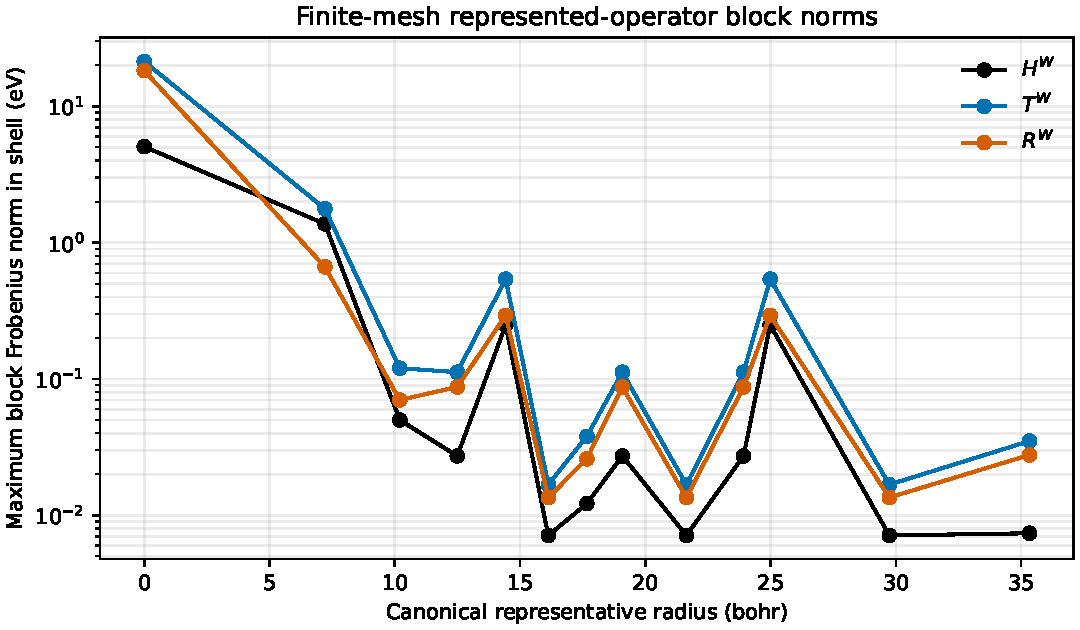
\includegraphics[width=0.93\linewidth]{../../../../../calculations/ICMSEP2026/conference/paper_1/silicon-wannier-kinetic-preview/real-space-shell-block-norms.pdf}
\caption{Component-resolved finite-mesh block norms for the read-only Wannier90 silicon
tutorial. Each point is the maximum Frobenius norm at one canonical representative
radius. The curves do not establish an infinite-lattice decay law.}
\label{fig:tutorial-blocks}
\end{figure}
A complete inverse finite transform contains 64 centered blocks. After retaining 57, the
maximum ordered-eigenvalue errors were:

\begin{table}[htbp]
\centering\small
\caption{Maximum ordered-eigenvalue errors after retaining 57 of 64 centered blocks.}
\label{tab:tutorial-errors}
\begin{tabularx}{0.72\textwidth}{XX}
\toprule
\textbf{Represented component} & \textbf{Maximum error} \\
\midrule
Total $H^W$ & 0.0207 eV \\
Kinetic $T^W$ & 0.0843 eV \\
Non-kinetic remainder $R^W$ & 0.0636 eV \\
\bottomrule
\end{tabularx}
\end{table}
All 64 blocks recovered the sampled matrices to roundoff. Table~\ref{tab:tutorial-errors}
and Fig.~\ref{fig:tutorial-truncation} therefore record a negative result for one
finite-mesh truncation, not a proof that every compact silicon Hamiltonian class fails.

\begin{figure}[htbp]
\centering
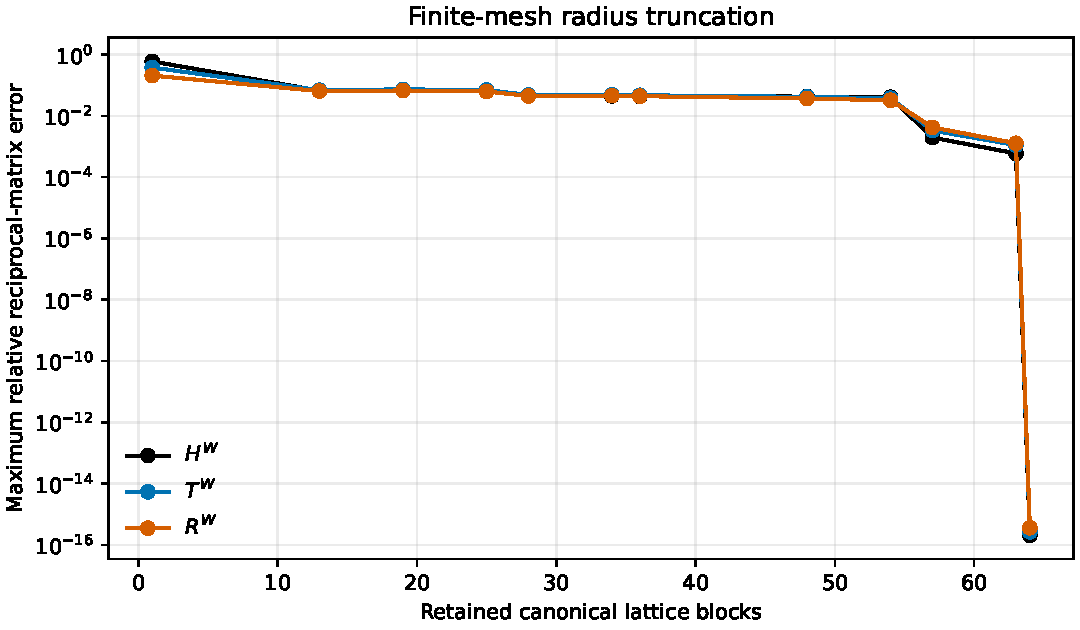
\includegraphics[width=0.93\linewidth]{../../../../../calculations/ICMSEP2026/conference/paper_1/silicon-wannier-kinetic-preview/real-space-truncation-relative-error.pdf}
\caption{Relative reciprocal-matrix errors under finite-block truncation for the
read-only tutorial representation. The final drop at 64 blocks is complete discrete
reconstruction, not continuum convergence.}
\label{fig:tutorial-truncation}
\end{figure}
\subsection{Evidence boundary}
Post-hoc SHA-256 correspondence confirms the tutorial input bytes but does not establish causal provenance for every source-run output. No Quantum ESPRESSO or Wannier90 run was repeated for this extraction. No independent reciprocal-mesh, cutoff, projector, effective-mass, or symmetry-alignment acceptance study is supplied.

This appendix may support statements about same-frame operator construction and failure of the tested 57-block truncation. It may not supply production settings, production thresholds, silicon effective masses, admissible-set membership, or model selection.

\end{document}
